\documentclass[dvipsnames,tikz]{standalone}
\usepackage{amsmath}
\usepackage{xcolor}
\usepackage{tikz}
\usetikzlibrary{calc}
\usetikzlibrary{decorations.pathreplacing,calligraphy,3d}
\usepackage{cmbright}      % sansfont


\begin{document}
	% add color=white for dark mode
	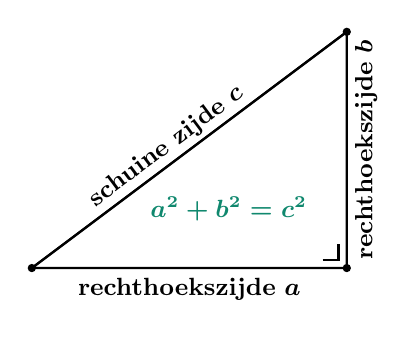
\begin{tikzpicture}[thick, color=black] 
		\draw (0,0) -- (4,0) -- (4,3) -- cycle;
		
		\draw[shift={(4,0)}, rotate=90, xshift=3pt, yshift=3pt] (0,0.2) -- (0,0) -- (0.2,0);
		
		\begin{scope}[font=\small]
			\fill (0,0) circle (1.5pt);
			\fill (4,0) circle (1.5pt);
			\fill (4,3) circle (1.5pt);
			\draw (2,0) node [below] {\textbf{rechthoekszijde} $\boldsymbol{a}$};
			\draw (4,0) -- node[sloped, midway, yshift=-7pt] {\textbf{rechthoekszijde} $\boldsymbol{b}$} (4,3);
			\draw (0,0) -- node[midway, sloped, xshift=-6pt, yshift=6pt] {\textbf{schuine zijde} $\boldsymbol{c}$} (4,3);
			
			\draw[PineGreen] (2.5,0.75) node {$\boldsymbol{a^2+b^2=c^2}$};
			
		\end{scope}
	\end{tikzpicture} 
	
\end{document}